% !TeX root = ../tesis.tex
%%%%%%%%%%%%%%%%%%%%%%%%%%%%%%%%%%%%%%%%%%%%%%%%%%%%%%%%%%%%%%%%%%%
% SECCIÓN: CAPAS DE CÓDIGO
%%%%%%%%%%%%%%%%%%%%%%%%%%%%%%%%%%%%%%%%%%%%%%%%%%%%%%%%%%%%%%%%%%%
\chapter{Capas de Código}
\label{ch:Capas-codigo}
% =============================================================================
%  SECCIÓN 4.1 — Filosofía de Arquitectura
% =============================================================================

\section{Filosofía de la Arquitectura: Hacia la democratización de la Tecnología de planeación}
\label{sec:filosofia-arquitectura}
La arquitectura computacional de esta investigación se fundamenta en la transición hacia herramientas de análisis de acceso abierto, 
rompiendo con la dependencia histórica de ecosistemas de software cerrados y onerosos para la administración pública. 
Históricamente, la planeación de redes de transporte ha estado supeditada al acceso a bases de datos comerciales, como NAVTEQ Map Data 
\parencite{navteq2012}, o al uso de plataformas SIG especializadas como TransCAD \parencite{caliper2010}, cuyos costos de licenciamiento y opacidad 
algorítmica imponen barreras de entrada significativas para los organismos locales.
Frente a este modelo, la democratización tecnológica se apoya en proyectos como OpenStreetMap (OSM) \parencite{osm2012}, que proporcionan capas 
de infraestructura vial libre, permitiendo una construcción transparente de grafos ruteables. Este enfoque se alinea con los preceptos de la \textbf{Free Software Foundation (FSF)}, 
la cual establece que la libertad del software radica en la capacidad de los usuarios para usar, estudiar, modificar y redistribuir las herramientas según las necesidades de la comunidad.
En términos de planeación urbana, la adopción de esta filosofía permite alcanzar una soberanía tecnológica, facilitando que las instituciones públicas acumulen capacidades analíticas autónomas 
y reduzcan la brecha de información en las periferias urbanas. Consecuentemente, el desarrollo de motores propios como \textbf{Apimetro} y \textbf{VFTModel}, basados en lenguajes de programación modernos como Go y Python, 
garantiza que el modelado y la optimización de la red multimodal de la ZMVM sea un proceso reproducible, transparente y accesible para el interés público.
\section{Apimetro: El motor de Datos metropolitano (Ingesta y ETL)}
\label{sec:apimetro-intro}

El proyecto \texttt{Apimetro} tiene su génesis entre los años 2023 y 2024, derivado de una necesidad cartográfica y de modelación espacial para el universo narrativo de \textbf{"La Saga de la Catacumba"}, obra del autor de la presente investigación. 
El primer volumen de esta serie, titulado \textbf{La historia de Quince}, explora una distopía urbana denominada "Ciudad Capital", la cual funciona como un homónimo especulativo de la Ciudad de México donde la habitabilidad se rige por la interacción crítica 
de tres variables: transporte, educación y tiempo. En dicha narrativa, el "tiempo" no es solo una dimensión física, sino un recurso de equidad social condicionado por la eficiencia de la infraestructura de movilidad. Para la construcción de este entorno literario, 
se requirió el desarrollo de un plan urbanístico que resolviera la fricción espacial de los protagonistas, quienes residían en polos opuestos de la metrópoli: el oriente y el sur profundo. En la realidad geográfica de la Ciudad de México, estas zonas corresponden a 
demarcaciones con un rezago histórico en transporte masivo, tales como Milpa Alta, Xochimilco, Tláhuac y Tlalpan. En estos sectores, la oferta de movilidad recae primordialmente en la \textbf{Red de Transporte de Pasajeros (RTP)}, 
cuya baja frecuencia y velocidades comerciales limitadas generaban, a nivel narrativo, "tiempos muertos" que dificultaban la fluidez de la trama. Esta problemática orilló a una convergencia multidisciplinaria que dio origen a cuatro proyectos paralelos: 
\textit{Apimetro}, \textit{La Catacumba}, \textit{VFTModel} y \textit{Diarios}.

La primera aproximación técnica para sistematizar la geografía metropolitana fue el desarrollo de \textit{"TrainMap"}, una herramienta de visualización que, aunque funcional 
para propósitos creativos, carecía del rigor matemático necesario para una auditoría urbana formal. A partir del año 2025, con el ingreso a la \textbf{Maestría en Urbanismo de la UNAM}, la investigación dio un giro hacia la formalización científica, 
integrando estándares como el \textit{General Transit Feed Specification} (GTFS) y sistemas de información geográfica (SIG).

\texttt{Apimetro} recibió una actualización estructural significativa a mediados de marzo de 2026, orientándose hacia un modelo de 
\textbf{Software as a Service (SaaS)} especializado en el manejo de tipos de datos \texttt{GeoJSON} para la representación cartográfica y el análisis ruteable. El núcleo operativo del sistema se define mediante un proceso \textbf{ETL}\footnote{En esta investigación se adopta la 
denominación \textit{Extraction, Treatment and Liberation} para enfatizar el carácter transformativo y de acceso abierto del proceso; el acrónimo estándar de la industria es \textit{Extract, Transform, Load}.},
diseñado para transformar la rigidez de los archivos \gtfs{} en geometrías flexibles. Si bien el estándar \gtfs{} posee una estructura relacional robusta, su formato original dificulta el análisis 
directo en hojas de cálculo o capas \texttt{SHP} convencionales, por lo que la conversión a \texttt{GeoJSON} se determinó como la solución más óptima para la visualización y el cálculo de indicadores topológicos. La persistencia y estructuración de la información 
se ejecutan dentro de una base de datos relacional \textbf{PostgreSQL 15}, potenciada por la extensión espacial \textbf{PostGIS 3.4}. Esta elección tecnológica permite almacenar datos geográficos de manera eficiente y proporciona operaciones de consulta avanzadas, 
como \texttt{ST\_AsGeoJSON} y \texttt{ST\_DWithin}, fundamentales para la ingesta y el ruteo asíncrono. Para la implementación de esta fase, se utilizó el lenguaje de programación \textbf{Python}, aprovechando la robustez de librerías especializadas en el manejo de 
grandes volúmenes de datos como \texttt{Pandas} y \texttt{PySpark}. Gracias a esta arquitectura, la ingesta de datos se consume de manera autosuficiente y óptima, resultando en una base de datos de apenas 38 MB en estado de desarrollo que es fácilmente replicable en 
diversos entornos operativos, incluyendo Linux, Windows, MacOS y plataformas web. Esta portabilidad facilita la auditoría de la red mediante gestores de consultas como \texttt{Postman} o su despliegue local a través de tecnologías de contenedores como \textbf{Docker} y 
\textbf{Docker Compose}. En última instancia, \texttt{Apimetro} garantiza la soberanía tecnológica de la investigación, permitiendo que la replicación del esquema de datos se realice de forma transparente mediante el archivo \texttt{seed.sql} disponible en su repositorio oficial.

\begin{figure}[htbp]
  \centering
  \includegraphics[width=0.45\textwidth]{Figures/Cap3/APImetroIcon.png}
  \caption[Ícono Personal de Apimetro]{Ícono Creado para el proyecto Apimetro}
  \label{fig:apimetro-icon}
  \fuentefigura{Elaboración propia.}
\end{figure}

\subsection{Modelo de Datos y Esquema Relacional}
\label{subsec:modelo-datos}

\subsubsection{Esquema Entidad-Relación E-R}
\label{subsubsec:EsquemaER}

El diseño del esquema relacional busca simplificar el estándar complejo del \gtfs{} (que incluye tablas como \textit{trips}, \textit{stop\_times} y \textit{shapes}) en tres entidades primordiales optimizadas para el consumo de la \api{} y el cálculo de indicadores topológicos:

\begin{figure}[H]
    \centering
    \includegraphics[width=0.85\textwidth]{Figures/Cap4/DiagramaER.png}
    \caption[Esquema Relacional Simplificado de Apimetro]{Representación de las entidades principales (Estaciones, Líneas y Polígonos) y sus relaciones para el cálculo de indicadores topológicos.}
    \label{fig:diagrama-er}
    \fuentefigura{Elaboración propia.}
\end{figure}


Como se observa en la Figura \ref{fig:diagrama-er}, el modelo se articula bajo los siguientes componentes:

\begin{itemize} 
    \item \textbf{Estaciones:} Nodo puntual que contiene atributos de conectividad y ubicación. 
    \item \textbf{Líneas:} Aristas de tipo \texttt{MultiLineString} que almacenan métricas operativas (velocidad, capacidad, frecuencia). 
    \item \textbf{Polígonos:} Áreas administrativas para filtrado por alcaldía o municipio. 
    \item \textbf{Relaciones:} Las líneas se vinculan con las estaciones a través de un identificador de sistema y ramal, permitiendo la reconstrucción del grafo metropolitano.
\end{itemize}


\subsubsection{Definición de Tablas Principales}
\label{subsubsec:DefinicionSQL}

El esquema relacional se implementa en tres tablas: \texttt{estaciones} (nodos puntuales con atributos de conectividad), \texttt{lineas} (aristas \texttt{MultiLineString} con métricas operativas de velocidad, frecuencia y capacidad) y \texttt{poligonos} (áreas administrativas para filtrado por alcaldía o municipio). Todas las columnas de geometría utilizan el tipo \texttt{GEOMETRY} con proyección WGS~84 (SRID~4326) e índices espaciales \texttt{GIST} para optimizar las consultas de ruteo. La definición completa del esquema \textsc{sql} se presenta en el Anexo~\ref{anx:apimetro-sql}.

La arquitectura de estas tablas responde a dos necesidades fundamentales identificadas en la investigación:
\begin{itemize}
    \item \textbf{Optimización de Consultas Geográficas:} El uso de columnas de tipo \texttt{GEOMETRY} y la creación de índices
    \texttt{GIST} permiten realizar operaciones espaciales masivas en milisegundos, tales como \texttt{ST\_AsGeoJSON} para la
    exportación de geometrías, \texttt{ST\_DWithin} para el cálculo de áreas de influencia o cobertura, y \texttt{ST\_Length} para
    determinar las distancias reales sobre la red vial.
    \item \textbf{Cálculo de Indicadores Operativos:} A diferencia de un \texttt{SIG}
    convencional, la tabla \texttt{lineas} integra atributos operativos críticos como la \textit{capacidad} del vehículo y la
    \textit{frecuencia} de paso. Esto permite que el motor \texttt{VFTModel} calcule automáticamente indicadores de desempeño como la
    \textbf{Fuerza Nodal ($C_i$)} y el \textbf{Tiempo de Viaje ($T$)}, ponderando el grafo metropolitano no solo por su fricción espacial,
    sino por la oferta real de transporte y las penalizaciones por transferencia.
\end{itemize}

Finalmente, es importante señalar que esta infraestructura está alineada con los preceptos de soberanía tecnológica y reproducibilidad
científica, siendo totalmente instalable en cualquier entorno (Docker, Linux, Windows o MacOS) mediante el archivo de inicialización
\texttt{init.sql} (o \texttt{seed.sql}) disponible en el repositorio oficial de \texttt{Apimetro} en GitHub.


\subsection{Tecnologías Backend}
\label{subsec:backend}
La arquitectura del motor de datos de la \zmvm se ha implementado utilizando el lenguaje de programación \textbf{Go 1.25}. 
La elección de esta tecnología no es fortuita; responde a la necesidad de procesar un grafo metropolitano con miles de nodos y aristas bajo condiciones 
de alta concurrencia y baja latencia. Go, al ser un lenguaje compilado, ofrece un rendimiento cercano a C++, pero con una gestión de memoria (\textit{Garbage Collection}) 
eficiente, lo cual es ideal para el ruteo asíncrono y el despacho de geometrías masivas en formato \texttt{GeoJSON}.
Para la capa de servicios web, se seleccionó el framework \textbf{Gin v1.9}. Gin se distingue por su enfoque minimalista y su velocidad en el ruteo de peticiones HTTP mediante 
un árbol de prefijos, lo que permite que los endpoints de \texttt{Apimetro} respondan en milisegundos incluso bajo cargas pesadas. El sistema se organiza bajo el patrón de diseño 
\textbf{MVC (Modelo-Vista-Controlador)}, permitiendo una separación clara entre la lógica de negocio, el dominio matemático y la persistencia de datos.

\subsubsection{Configuración y Entorno de Ejecución}
\label{subsubsec:configuracionejecucion}

Para garantizar la portabilidad y soberanía tecnológica, el backend se configura mediante variables de entorno que permiten su despliegue en contenedores \textbf{Docker}. Las variables críticas cubren la conexión al motor espacial (\texttt{DB\_HOST}, \texttt{DATABASE\_URL}) y el modo de ejecución del framework (\texttt{GIN\_MODE}); su especificación completa se presenta en el Cuadro~\ref{tab:env-vars} del Anexo~\ref{anx:apimetro-backend}.

\subsubsection{Estructura de Endpoints y Lógica de Respuesta}
\label{subsubsec:estructuraEndpoints}
La capa de rutas de \texttt{Apimetro} expone la interfaz pública del sistema, actuando como el punto de entrada para el consumo de datos georreferenciados. 
Todos los endpoints de mapas han sido diseñados para devolver objetos de tipo \texttt{FeatureCollection} bajo el estándar \textbf{GeoJSON RFC 7946} \parencite{cabrera2025apimetro}. 
Esta arquitectura permite que el sistema opere bajo un modelo de \textbf{SaaS (Software as a Service)}, donde clientes analíticos como \textit{VFTModel} o visores 
cartográficos consumen datos ya normalizados y ruteables. Esto elimina la necesidad de procesar los archivos de texto plano de los feeds \gtfs{} originales en cada consulta, 
optimizando significativamente el rendimiento computacional al calcular indicadores como el \textbf{Tiempo de Viaje Promedio (T)} y el \textbf{Índice de Ruta Directa (DI)} \parencite{cabrera2026VFTModel}.

Para ejemplificar la versatilidad del backend desarrollado en \textbf{Go}, se analizan las dos estructuras principales del sistema: la gestión de nodos puntuales (estaciones) y la recuperación de geometrías 
complejas (líneas y ramales).
\paragraph{Control de Estaciones (Nodos):} El controlador \texttt{estaciones.go} gestiona la lógica de filtrado de las paradas del sistema metropolitano capturando parámetros dinámicos de la \textsc{url} (sistema, alcaldía, jerarquía de transporte) para segmentar la red y permitir auditorías locales precisas. El código fuente completo se presenta en el Anexo~\ref{anx:apimetro-backend}.

\paragraph{Optimización de Indicadores:}
La separación de estas lógicas en controladores especializados permite que una petición de ruteo para el \textbf{Tercer Contorno} sea resuelta mediante índices espaciales \texttt{GIST} en milisegundos \parencite{cabrera2025apimetro}.

Esta estructura garantiza que la planeación urbana no dependa de la manipulación manual de datos pesados, permitiendo que la simulación de escenarios de transporte sea un proceso dinámico, 
reproducible y basado en la soberanía tecnológica de herramientas de código abierto \parencite{cabrera2025apimetro}.


\subsection{Salidas Estructurales (GeoJSON)}
\label{subsec:estructura-geojson}

La elección del formato de intercambio de datos geoespaciales constituye una decisión crítica para la operatividad de los sistemas de transporte modernos. En el desarrollo del motor \texttt{Apimetro}, se ha priorizado
 el uso del estándar \textbf{GeoJSON (RFC 7946)} sobre el formato tradicional \textit{ESRI Shapefile} (SHP). Mientras que el formato SHP representa un estándar de legado que requiere una colección de múltiples archivos 
independientes (\textit{.shp, .dbf, .shx}) para su funcionamiento y presenta limitaciones de codificación en entornos web, el GeoJSON es un formato basado íntegramente en texto plano (\textit{JSON}) diseñado 
específicamente para la transferencia ágil de datos geográficos en aplicaciones móviles y sistemas distribuidos \parencite{cabrera2025apimetro}.

Una de las ventajas determinantes de este formato es su \textbf{compatibilidad nativa} con las librerías de mapas de alto rendimiento más utilizadas en la industria tecnológica, tales como \textit{Leaflet}, 
\textit{Mapbox} y \textit{MapLibre} \parencite{cabrera2025apimetro}. Esta característica permite que los datos de movilidad de la \zmvm se integren directamente en visores interactivos sin necesidad de 
realizar transformaciones pesadas en el lado del cliente o recurrir a servidores de mapas intermediarios. Al ser un estándar basado en texto, facilita la transparencia en la auditoría de los datos y 
asegura la soberanía tecnológica de la investigación al utilizar insumos oficiales de acceso abierto \parencite{adip_gtfs_2024}.

Asimismo, la integración de GeoJSON con bases de datos espaciales como \textbf{PostGIS} permite que la generación de mapas sea un proceso dinámico y asíncrono. Mediante funciones nativas de conversión, el sistema 
transforma la topología de la red almacenada en tablas de estaciones y líneas en geometrías ruteables de forma inmediata \parencite{fortin2016innovative}. 
Este enfoque supera la rigidez de los archivos vectoriales estáticos, permitiendo que cada objeto geográfico transporte, dentro de su estructura de \textit{properties}, no solo su ubicación espacial sino 
también sus métricas operativas críticas —como velocidad promedio, frecuencia y capacidad del vehículo—. Esta consolidación de información en un solo objeto estructurado es fundamental para el procesamiento 
analítico del motor \textit{VFTModel} al evaluar la eficiencia de la red \parencite{cabrera2026VFTModel}.

\subsection{Estructura de JSON Descriptivo (No Geográfico)}
\label{subsec:estructura-geojson-descriptivo}

Complementariamente a las salidas espaciales, el motor \texttt{Apimetro} provee una capa de \textbf{respuestas descriptivas} en formato JSON estándar. Esta estructura está diseñada específicamente para gestionar atributos 
alfanuméricos, metadatos históricos y parámetros de estilo que no requieren de una representación geométrica inmediata para su procesamiento \parencite{cabrera2025apimetro}. 
La utilidad de esta salida radica en su eficiencia para alimentar componentes de interfaz de usuario, tales como fichas técnicas de estaciones, tablas de atributos operativos o la configuración de la simbología visual 
en visores cartográficos sin incurrir en el costo computacional de transferir coordenadas geográficas masivas.

A diferencia del estándar GeoJSON, orientado al renderizado de mapas, el JSON descriptivo permite realizar consultas rápidas sobre la jerarquía administrativa y la cronología del sistema de transporte~\parencite{cabrera2025apimetro}. Estos registros vinculan la información operativa almacenada en la tabla \texttt{historico\_operacion} con las identidades comerciales de cada línea. Un ejemplo representativo de esta salida se presenta en el Anexo~\ref{anx:apimetro-salidas}.

Entre los campos de mayor relevancia para la planeación se encuentran \texttt{color\_esp} —que permite la estandarización visual de las rutas bajo los lineamientos oficiales de identidad institucional de la \zmvm{}— y \texttt{clasificacion} —que distingue entre infraestructura existente, futura o eliminada—, ambos fundamentales para que el motor \textit{VFTModel} realice comparaciones estadísticas entre la red actual y los escenarios de expansión propuestos~\parencite{cabrera2026VFTModel, adip_gtfs_2024}. Esta separación de intereses entre los datos descriptivos y los geográficos asegura que el flujo de información sea escalable y se adapte a las necesidades específicas de la planeación urbana estratégica y la auditoría de redes complejas~\parencite{fortin2016innovative}.

\subsection{Estructura de GeoJSON (Geográfico)}
\label{subsec:estructura-geojson-geografico}

La salida geográfica de \texttt{Apimetro} constituye la columna vertebral del sistema, transformando la persistencia relacional de la base de datos en objetos espaciales listos para el análisis y la visualización \parencite{cabrera2025apimetro}. 
A diferencia de los formatos tabulares, la estructura GeoJSON permite una jerarquía anidada que encapsula la topología de la red metropolitana en un solo archivo de texto plano. A continuación, se describen los cuatro componentes fundamentales 
que integran cada respuesta del motor:

\paragraph{1. FeatureCollection:} Es el contenedor de nivel superior que agrupa un conjunto de entidades geográficas. En el contexto de esta investigación, un \texttt{FeatureCollection} puede representar la totalidad de las estaciones de un sistema 
(como el Metrobús) o el trazo completo de un ramal operativo.

\paragraph{2. Feature:} Representa una unidad individual dentro de la red, ya sea un nodo puntual (estación) o una arista (segmento de línea). Cada \texttt{Feature} actúa como el vínculo entre la geometría física y sus atributos descriptivos.

\paragraph{3. Geometry:} Define el componente espacial de la entidad utilizando coordenadas geográficas bajo el elipsoide \textbf{WGS 84 (SRID 4326)}. \texttt{Apimetro} emplea primordialmente dos tipos de geometrías: 
\texttt{Point} para la geolocalización exacta de estaciones y paradas, y \texttt{MultiLineString} para representar los trazos de las rutas, permitiendo capturar la continuidad de la infraestructura vial incluso en segmentos fragmentados.

\paragraph{4. Properties:} Es el objeto donde se almacena la metadata enriquecida y las métricas operativas. En esta sección, el motor integra datos como la \texttt{alcaldia\_municipio}, el \texttt{sistema}, y variables críticas para el motor \textit{VFTModel} 
como la \texttt{velocidad\_promedio\_kmh} y la \texttt{frecuencia\_minutos}.

Un ejemplo representativo de la estructura de una estación de transporte masivo generada por la \api{} se presenta en el Anexo~\ref{anx:apimetro-salidas}.

La propiedad \texttt{coordinates} proporciona la base para el cálculo de la \textbf{Distancia Euclidiana} necesaria para obtener el \textbf{Índice de Ruta Directa ($DI$)}. Al mismo tiempo, las \texttt{properties} permiten realizar filtrados dinámicos en el lado del cliente, facilitando que aplicaciones móviles o visores web presenten únicamente la información relevante para la planeación del corredor anillar propuesto \parencite{cabrera2025apimetro, adip_gtfs_2024}. Esta arquitectura asegura que la información geográfica no sea solo una representación visual, sino un insumo matemático auditable y reproducible \parencite{fortin2016innovative}.
\subsection{El Futuro de Apimetro}
\label{subsec:futuro-apimetro}

\texttt{Apimetro} se define no solo como una herramienta técnica, sino como un proyecto de \textbf{software libre} comprometido con la democratización de los datos de movilidad en la \zmvm. Bajo la premisa de soberanía tecnológica, 
el proyecto se encuentra en una fase de expansión activa, proyectando un crecimiento significativo en su cobertura y capacidades analíticas en los próximos meses \parencite{cabrera2025apimetro}. 
Para facilitar la transparencia, el estudio y la redistribución del conocimiento generado, el ecosistema de \texttt{Apimetro} se articula a través de cuatro plataformas principales:

\paragraph{1. Página Oficial (apimetro.dev):} Es el punto de entrada principal para usuarios y desarrolladores. En este portal se aloja la documentación interactiva (Swagger UI), el estado de salud del servidor de producción y los 
accesos rápidos a los recursos de la API masiva.

\begin{figure}[htbp]
  \centering
  \includegraphics[width=0.85\textwidth]{Figures/Cap3/PantallaInicialApimetro.png}
  \caption{Interfaz principal del portal \url{apimetro.dev}.}
  \label{fig:screenshot-web}
\end{figure}

\paragraph{2. Repositorio de Código en GitHub:} Constituye el núcleo técnico del proyecto. Aquí se encuentra el código fuente en \textbf{Go}, los motores de ingesta \textbf{ETL} y las configuraciones de despliegue mediante \textbf{Docker}. 
El repositorio está bajo una licencia \textit{Business Source License 1.1}, la cual garantiza su uso gratuito para fines académicos, de investigación y del sector público, con una transición automática a la licencia \textit{Apache 2.0} 
en abril de 2029 \parencite{cabrera2025apimetro}.

\begin{figure}[htbp]
  \centering
  \includegraphics[width=0.85\textwidth]{Figures/Cap3/PantallaInicialApimetroGithub.png}
  \caption{Estructura del c{\'o}digo fuente y control de versiones en GitHub.}
  \label{fig:screenshot-repo}
\end{figure}

\paragraph{3. Comunidad de Desarrollo (Discussions):} Espacio dedicado a la colaboración abierta y la gobernanza del proyecto. A través de este canal, la comunidad puede proponer nuevas funcionalidades, reportar incidencias en los trazos 
de transporte o discutir la integración de nuevos sistemas de la Zona Metropolitana, fomentando una construcción colectiva de la infraestructura de datos.

\begin{figure}[htbp]
  \centering
  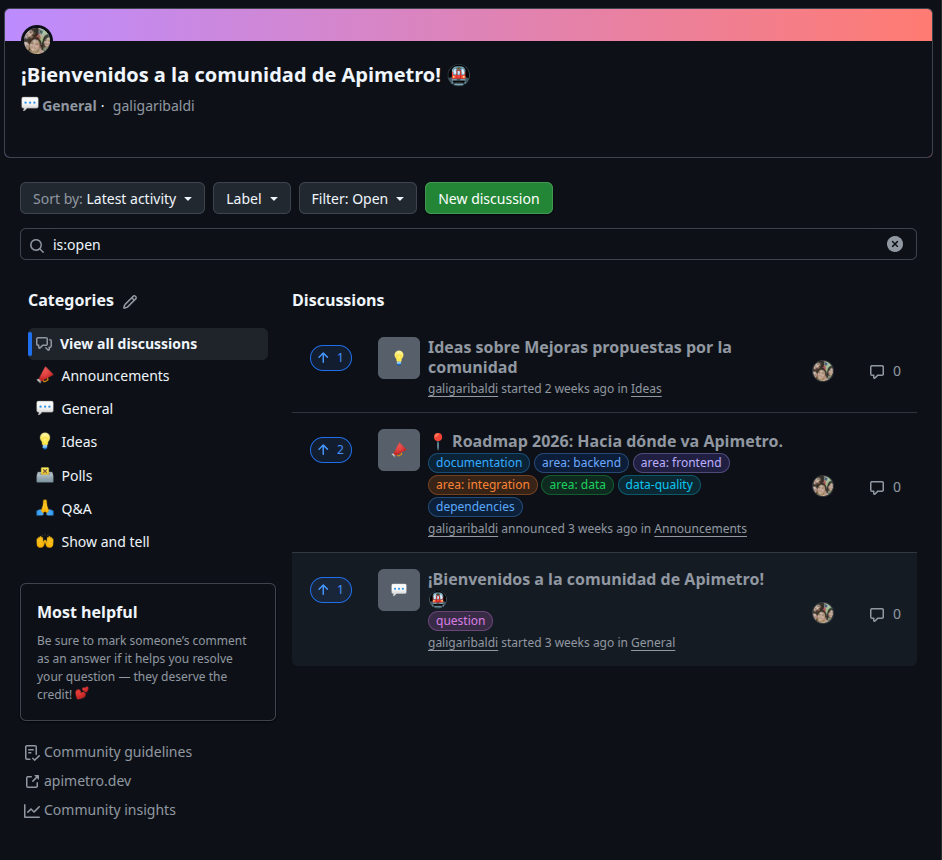
\includegraphics[width=0.85\textwidth]{Figures/Cap3/PantallaInicialComunidadApimetro.png}
  \caption{Foro de discusi{\'o}n y colaboraci{\'o}n de la comunidad Apimetro.}
  \label{fig:screenshot-discussions}
\end{figure}

\paragraph{4. Wiki de Apimetro:} Centro de documentación técnica profunda donde se detallan las guías de implementación, el diccionario de datos de las tablas \texttt{SQL} y los procedimientos para replicar el motor de datos de forma local 
utilizando el archivo \texttt{seed.sql}.

\begin{figure}[htbp]
  \centering
  \includegraphics[width=0.85\textwidth]{Figures/Cap3/PantallawikiApimetro.png}
  \caption{Repositorio de documentaci{\'o}n t{\'e}cnica y gu{\'i}as de implementaci{\'o}n.}
  \label{fig:screenshot-wiki}
\end{figure}

Esta infraestructura digital asegura que la investigación no termine con la entrega de la tesis, sino que perdure como un \textbf{bien público tecnológico} capaz de evolucionar y adaptarse a las dinámicas cambiantes de la movilidad 
urbana en México \parencite{fortin2016innovative}.